\documentclass[11pt, oneside]{article} 
\usepackage{geometry}
\geometry{letterpaper} 
\usepackage{graphicx}
	
\usepackage{amssymb}
\usepackage{amsmath}
\usepackage{parskip}
\usepackage{color}
\usepackage{hyperref}

%\graphicspath{{/Users/telliott_admin/Tex/png/}}
\graphicspath{{/Users/telliott_admin/Desktop}}
% \begin{center} 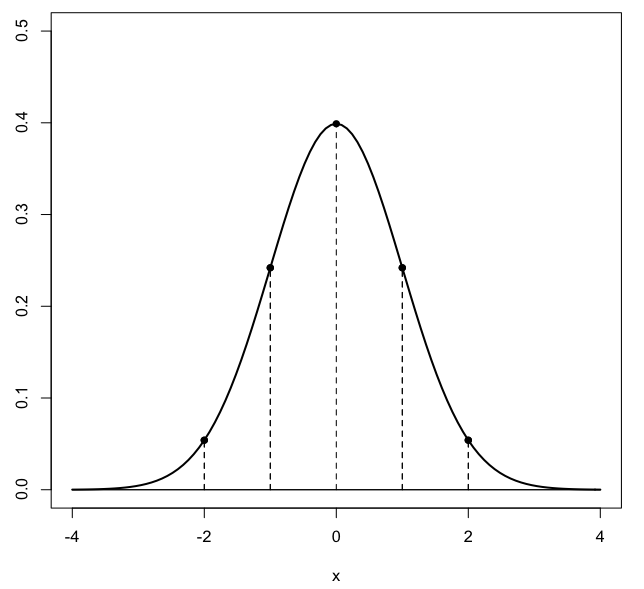
\includegraphics [scale=0.4] {gauss3.png} \end{center}

\title{Shearer problems}
\date{}

\begin{document}
\maketitle
\Large
\subsection*{problem 1}
 \begin{center} 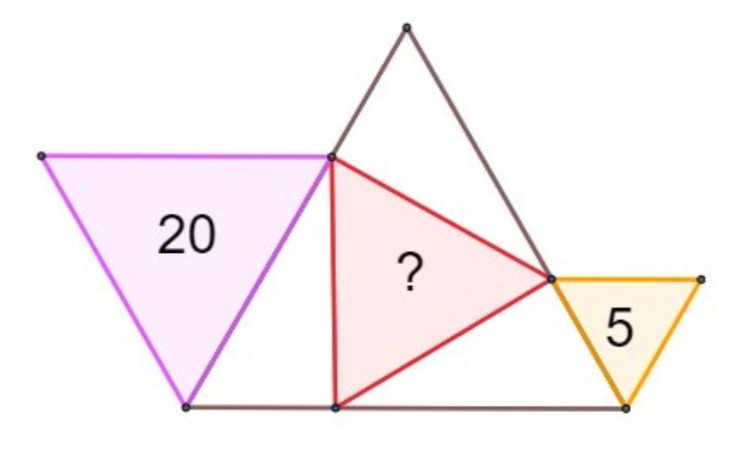
\includegraphics [scale=0.3] {Shearer1.png} \end{center}
The numbers look like areas.  Assume we have 4 equilateral triangles. Let $h$ be the height of the one on the left.  Then $h/b = \sqrt{3}/2$.
\[ A = 20 = \frac{1}{2} \ hb = \frac{1}{\sqrt{3}} \ h^2 \]

\end{document}